
\paragraph{3. Presence of cycles?}
    Before we go into analyzing whether new relations introduce observable behaviours, we first ensure there are no $\stck{_\textit{hb}}$ cycles introduced in the process. This is because the model requires that $\stck{_{hb}}$ is a strict partial order. 
    
    Note that if a cycle exists after reordering, then 
    \begin{enumerate}
        \item The relations preserved do not themselves create a cycle (ref to the theorem)
        \item Additional new relations may introduce cycles
    \end{enumerate}

    The first part is straightforward as we assume we can only do reordering on Candidate Exectuions of $C$ not having happens-before cycles. 
    For the second part, we first address the cases where $\reln{d}{hb}{e}$ may be part of the cycle. 
    The other event $k$, may be either from the set $K_e$, $K_d$ or a new relation that is formed\footnotemark.

    \footnotetext{$K_e$ and $K_d$ only apart from the new relation because these are the only valid cases where happens-before relations are preserved after reordering. So we need not consider cases such thta $\reln{e}{hb}{k}$ or $\reln{k}{hb}{d}$ as the old relations they are covered by $K_e$ and $K_d$.}
    
    Figure~\ref{reord:cycle(a)} shows that $k$ cannot belong to either of the sets, as their relations with $e$ and $d$ will not result in a cycle. 
    \begin{figure}[H]
        \centering
        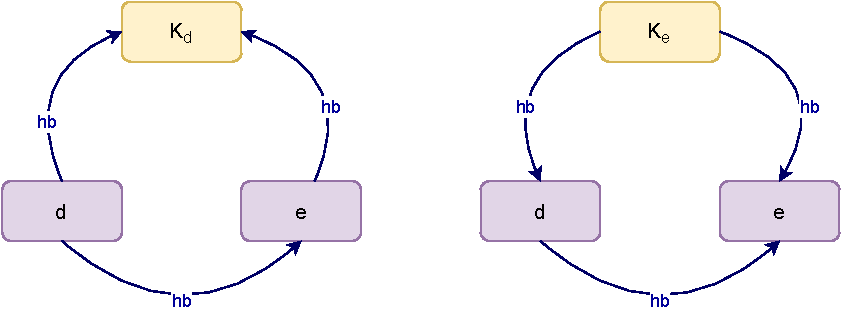
\includegraphics[scale=0.7]{5.InstructionReordering/4.ValidReorderingCandidate/ProofParts/Part3/part3(b).pdf}
        \caption{If event $k$ is from $K_e$ or $K_d$, there are not happens-before cycles.}
        \label{reord:cycle(a)}
    \end{figure}

    For cases where $\reln{k}{hb}{e}$ is the set of new relations, note that by lemma 1
    \[
        \reln{k}{hb}{e} \Rightarrow \reln{k}{hb}{d}
    \]

    For cases where $\reln{d}{hb}{k}$ is the set of new relations, by lemma 2
    \[
        \reln{d}{hb}{k} \Rightarrow \reln{e}{hb}{k}
    \]

    So for both these cases also, a cycle with $\reln{d}{hb}{e}$ cannot exist. 
    Figure~\ref{reord:cycle(b)} shows pictorially this fact. 
    \begin{figure}[H]
        \centering
        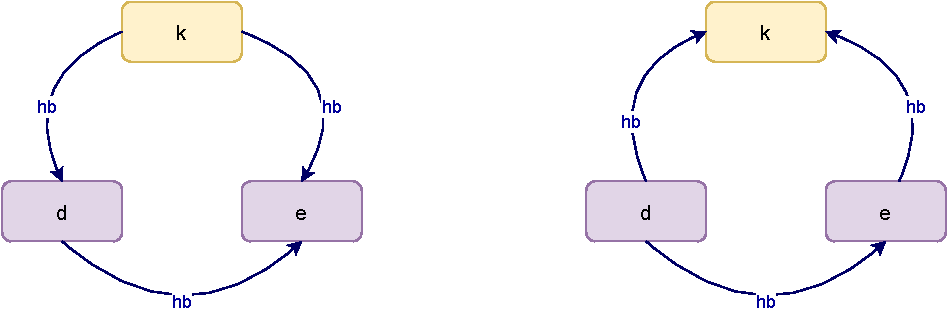
\includegraphics[scale=0.7]{5.InstructionReordering/4.ValidReorderingCandidate/ProofParts/Part3/part3(c).pdf}
        \caption{Sets of relations $\reln{k}{hb}{e}$ or $\reln{d}{hb}{k}$ individually do not create any cycles.}
        \label{reord:cycle(b)}
    \end{figure}

    For the one case where we have two new sets of relations formed, i.e $\reln{d}{hb}{k}$ and $\reln{k}{hb}{e}$, we could have a case where $k$ is a common event for both sets. But, by Lemma \ref{Lemma1}, we also have $\reln{k}{hb}{d}$ and by Lemma \ref{Lemma2}, $\reln{e}{hb}{k}$\footnotemark. Thus, we have a cycle. Figure~\ref{reord:cycle(c)} below shows this pictorially.
    \begin{figure}[H]
        \centering
        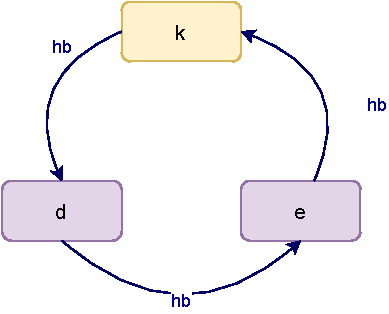
\includegraphics[scale=0.7]{5.InstructionReordering/4.ValidReorderingCandidate/ProofParts/Part3/part3(d).pdf}
        \caption{Sets of relations $\reln{k}{hb}{e}$ and $\reln{d}{hb}{k}$ creates a cycle.}
        \label{reord:cycle(c)}
    \end{figure}

    \footnotetext{It is not actually due to lemmas, but just that the new relations were derived through $e$ or $d$, as these relations existed before reordering.}

    Now for the case when $\reln{d}{hb}{e}$ may not be part of the cycle, we have only two other new relations, $\reln{k}{hb}{e}$ or $\reln{d}{hb}{k}$.

    Considering the first scenario where the new set of relations are of the form $\reln{k}{hb}{e}$. Suppose a cycle exists with another event $k'$. Then 
    \[
        \reln{k}{hb}{e} \ \wedge \
        \reln{e}{hb}{k'} \ \wedge \
        \reln{k'}{hb}{k}
    \]

    Note that the latter two relations are not new, since the only new set of relations are of the first form. Now, by Lemma \ref{Lemma1} and by transitivity respectively
    \begin{gather*}
        \reln{k}{hb}{e} \Rightarrow \reln{k}{hb}{d} \\
        \reln{e}{hb}{k'} \Rightarrow \reln{d}{hb}{k'}    
    \end{gather*}

    So, the following is also a cycle
    \[
        \reln{k}{hb}{d} \ \wedge \
        \reln{d}{hb}{k'} \ \wedge \
        \reln{k'}{hb}{k}
    \]

    But these relations already exist in the original Candidate Execution, which implies a cycle existed before reordering. This contradicts our assumption that we only reorder when the Candidate Executions of $C$ have no cycles. Thus, by contradiction such a cycle cannot exist.

    In similar lines for the cases where the set of new relations are of the form $\reln{d}{hb}{k}$,  Suppose a cycle exists with another event $k'$. Then 
    \begin{align*}
        \reln{d}{hb}{k} \ \wedge \
        \reln{k}{hb}{k'} \ \wedge \ 
        \reln{k'}{hb}{d} 
    \end{align*}

    Note that the latter two relations are not new, since the only new set of relations are of the first form. Now, by Lemma \ref{Lemma2} and by transitivity respectively, we have 
    \begin{align*}
        \reln{d}{hb}{k} \Rightarrow \reln{e}{hb}{k}
        \reln{k'}{hb}{d} \Rightarrow \reln{k'}{hb}{d}
    \end{align*}

    Thus, we also have the cycle 
    \begin{align*}
        \reln{e}{hb}{k} \ \wedge \
        \reln{k}{hb}{k'} \ \wedge \ 
        \reln{k'}{hb}{e} 
    \end{align*}

    But these relations already exist in the original Candidate Execution, which implies a cycle existed before reordering. This contradicts our assumption that we only reorder when the Candidate Executions of $C$ have no cycles. Thus, by contradiction such a cycle cannot exist.

    Figure~\ref{reord:cycle_table} shows the cases where new relations have no happens-before cycles. 
    \begin{figure}[H]
        \centering
        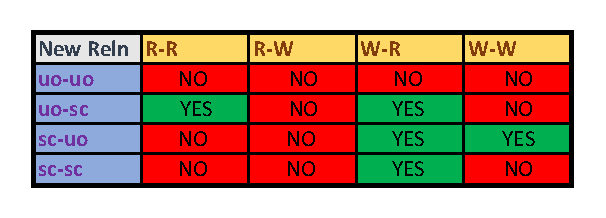
\includegraphics[scale=0.7]{5.InstructionReordering/4.ValidReorderingCandidate/ProofParts/Part3/part3_table.pdf}
        \caption{Table summarizing \textit{happens-bfore} cycles that may be introduced after reordernig candidates with valid pivots.}
        \label{reord:cycle_table}
    \end{figure}